\documentclass[12pt]{report}

\usepackage{listings} % used to insert code snippets
\usepackage{xcolor} % used to include specific colors
\usepackage{longtable}
\usepackage{textcomp}
\usepackage{subfig}
\usepackage{graphicx}
\usepackage{cleveref}
\usepackage{bm}

\lstset{breaklines=true}

% These are the appendices
\begin{document}

\appendix
\chapter{List of Parameters\label{app:params}}

\begin{longtable}{r l l}
\label{table:params}\\
\caption{This table gives the parameters for UO\textsubscript{2} generating the energy function.}\\
\hline
\hline
Array number & Parameter name & Parameter value \\
\hline
\endfirsthead
\multicolumn{3}{c}{\tablename\ \thetable\ -- \textit{Continued from previous page}}\\
\hline
Array number & Parameter name & Parameter value \\
\hline
\endhead
\hline
\multicolumn{3}{r}{\textit{Continued on next page.}}\\
\endfoot
\hline
\hline
\endlastfoot
1 & Energy Scaling Factor ($e_{RGB}$) & 1.6012 $J/m^2$ \\
2 & \textlangle{}100\textrangle{} Max Distance & 0.405 \\
3 & \textlangle{}110\textrangle{} Max Distance & 0.739 \\
4 & \textlangle{}111\textrangle{} Max Distance & 0.352 \\
5 & \textlangle{}100\textrangle{} Weight & 50.5 \\
6 & \textlangle{}110\textrangle{} Weight & 4.55 \\
7 & \textlangle{}111\textrangle{} Weight & 0.08 \\
8 & \textlangle{}100\textrangle{} Tilt/Twist Mix Power Law (1) & 0.03325 \\
9 & \textlangle{}100\textrangle{} Tilt/Twist Mix Power Law (2) & 0.00053125 \\
10 & Maximum \textlangle{}100\textrangle{} Twist Energy & 0.60903 \\
11 & \textlangle{}100\textrangle{} Twist Shape Factor & 1.4486 \\
12 & \textlangle{}100\textrangle{} Asymmetric Tilt Interpolation Power & 35.8 \\
13 & \textlangle{}100\textrangle{} Symmetric Tilt First Peak Energy & 1.0058 \\
14 & \textlangle{}100\textrangle{} Symmetric Tilt First $\Sigma5$ Energy & 0.84456 \\
15 & \textlangle{}100\textrangle{} Symmetric Tilt Second Peak Energy & 0.97259 \\
16 & \textlangle{}100\textrangle{} Symmetric Tilt Second $\Sigma5$ Energy & 0.9379 \\
17 & \textlangle{}100\textrangle{} Symmetric Tilt $\Sigma17$ Energy & 0.96881 \\
18 & \textlangle{}100\textrangle{} Symmetric Tilt First Peak Angle & 0.31569 \\
19 & \textlangle{}100\textrangle{} Symmetric Tilt Second Peak Angle & 0.88538 \\
20 & \textlangle{}110\textrangle{} Tilt/Twist Mix Power Law (1) & 3.1573 \\
21 & \textlangle{}110\textrangle{} Tilt/Twist Mix Power Law (2) & 1.9784 \\
22 & \textlangle{}110\textrangle{} Twist Peak Angle & 0.46145 \\
23 & \textlangle{}110\textrangle{} Twist Peak Energy & 1.1444 \\
24 & \textlangle{}110\textrangle{} Twist $\Sigma3$ Energy & 1.0931 \\
25 & \textlangle{}110\textrangle{} Twist 90\textdegree{} Energy & 1.152 \\
26 & \textlangle{}110\textrangle{} Asymmetric Tilt Shape Factor & 3.1843 \\
27 & \textlangle{}110\textrangle{} Symmetric Tilt Third Peak Energy & 1.0514 \\
28 & \textlangle{}110\textrangle{} Symmetric Tilt $\Sigma3$ Energy & 0.61703 \\
29 & \textlangle{}110\textrangle{} Symmetric Tilt Second Peak Energy & 1.0902 \\
30 & \textlangle{}110\textrangle{} Symmetric Tilt $\Sigma11$ Energy & 0.56686 \\
31 & \textlangle{}110\textrangle{} Symmetric Tilt First Peak Energy & 1.1024 \\
32 & \textlangle{}110\textrangle{} Symmetric Tilt Third Peak Angle & 0.88736 \\
33 & \textlangle{}110\textrangle{} Symmetric Tilt Second Peak Angle & 1.8711 \\
34 & \textlangle{}110\textrangle{} Symmetric Tilt First Peak Angle & 2.731 \\
35 & \textlangle{}111\textrangle{} Tilt-Twist Linear Interpolation & 38.201 \\
36 & \textlangle{}111\textrangle{} Twist Shape Factor & 1.2414 \\
37 & \textlangle{}111\textrangle{} Twist Peak Angle & 0.49979 \\
38 & \textlangle{}111\textrangle{} Twist Peak Energy & 0.7971 \\
39 & \textlangle{}111\textrangle{} Symmetric Tilt Peak Angle & 0.25966 \\
40 & \textlangle{}111\textrangle{} Symmetric Tilt Max Energy & 1.0288 \\
41 & \textlangle{}111\textrangle{} Symmetric Tilt $\Sigma3$ Energy & 1.1311 \\
42 & \textlangle{}111\textrangle{} Asymmetric Tilt Symmetry Point Energy & 3.7674 \\
43 & \textlangle{}111\textrangle{} Asymmetric Tilt Scale Factor & 0.053417 \\
\end{longtable}

\chapter{Grain Boundary Representations\label{app:gbRep}}
Visual representations of the GB space helped Bulatov \emph{et al.} develop their 5D function.  However, the size of the five-space in which GBs reside makes representing them difficult.  Researchers have developed different methods to represent them, each with their advantages and disadvantages.  Three of these methods are the axis-angle representation, the Rodrigues representation, and the fundamental zone representation.  These methods, though described separately, can be used together to form a better picture of what the GB space looks like (see for example \Cref{fig:bulatovRodrigues} which combines the Rodrigues representation and the fundamental zone representation).

\section{Axis-Angle Representation\label{GBReps:AA}}
Of the three described, the axis-angle representation most simplistically describes GB space.  The axis of rotation of the GB specifies the point in axis-angle space, and the angle of misorientation between the two grains at the GB specifies the magnitude of the vector.  Thus, the axis ($\bm{a}$, where $\bm{a}$ has components $a_x$, $a_y$, and $a_z$) and the angle ($\theta$) mathematically represent an axis-angle vector as:
\begin{equation}
\bm{A} = \bm{a}\ \theta
\label{eq:aaVec}
\end{equation} 

The axis-angle space can only take into account three degrees of freedom: the two angles specifying the axis, and the angle rotated through.  Thus, axis-angle space cannot fully visualize all of the necessary information contained in the full 5D space.\cite{frank1988} This representation suffers from the difficulties of understanding an infinite space because it maps an axis and an angle onto a Cartesian coordinate system.  Without the help of additional methods, this infinite space remains difficuly to understand.  The best uses of this representation focus on using it as a starting point to move to other, more robust representations, and to represent the misorientation between two grains.\cite{randle2000}

\section{Rodrigues Representation\label{GBReps:Rodrigues}}
The Rodrigues representation (sometimes called the ``Rodrigues-Frank" representation) uses Rodrigues vectors to represent rotations in Rodrigues space.  This representation takes ideas from the axis-angle space, but makes a few changes allowing crystal symmetries to be taken into account.  The orientation of the GB normal still specifies the point in space, but the tangent of half the angle represents the magnitude of the vector. Thus, a Rodrigues vector can be represented as:\cite{morawiec1996, becker1989, frank1988, randle2000, priester2013}
\begin{equation}
\bm{R}=\bm{a}\ \textnormal{tan}\left(\frac{\theta}{2}\right)
\label{eq:rodriguesVec}
\end{equation}
Some researchers favor this representation over others because of the lack of curvature such a mapping entails.\cite{frank1988, randle2000}  However, it still only specifies three of the five degrees of freedom.  Bulatov \emph{et al.}\ attached a unit vector at the points along the axis to represent the other two DoFs in \Cref{fig:bulatovRodrigues}. A parallel vector represents a twist boundary, and a perpendicular vector represents a tilt boundary.  Anything else represents a mix of twist and tilt (or a mixed boundary).  One limitation of Rodrigues space lies in that it also maps to an infinite space.\cite{frank1988, kirch2008}.

\section{Fundamental Zone Representation\label{GBReps:FunZone}}
The fundamental zone best graphically represents the full 5D GB.  This representation takes advantage of the symmetries inherent in crystals\cite{stokes2007} to simplify an infinite space into a compact, finite area called the fundamental zone.\cite{bulatov2014, patala2013, homer2015, morawiec1996, patala2012}  Every point within the space represents a unique orientation, and every point outside the space can be represented as a point inside the space through symmetry operations.\cite{morawiec1996, becker1989, frank1988}  Bulatov \emph{et al.}\ used this idea in connection with Rodrigues space to create \Cref{fig:bulatovRodrigues}.  In Rodrigues space, the crystal symmetries of the material determine the shape of the fundamental zone.\cite{patala2013, morawiec1996}  For fcc crystals, the fundamental zone takes the form of a truncated tetrahedron.\cite{bulatov2014}  The edges of the fundamental zone in Rodrigues space represent the high-symmetry rotation axes, and points on one face can represent another point on a different face of the fundamental zone.  

\chapter{Graphs\label{app:graphs}}
\begin{figure}[ht!]
 \centering
 
 \subfloat[]{\label{appfig:compare100Twist}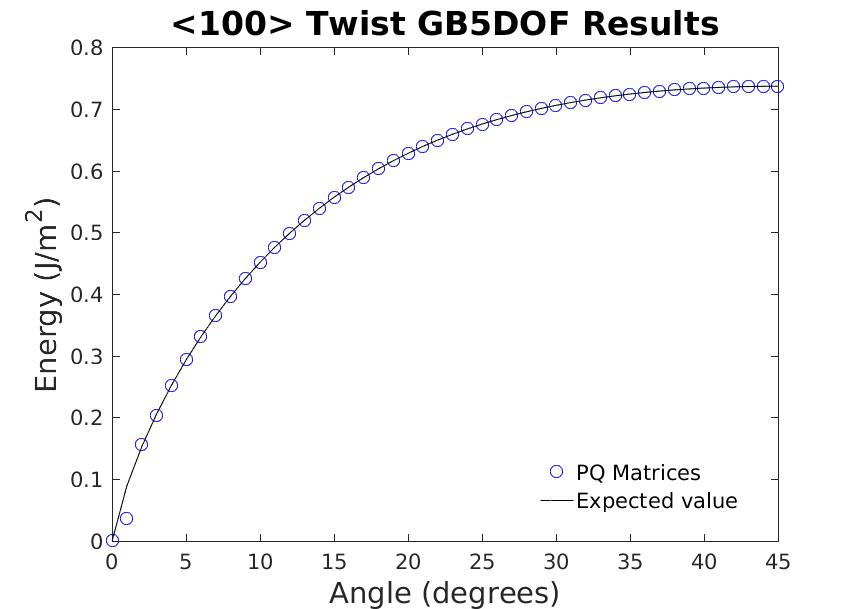
\includegraphics[scale=0.24]{Images/TestPQFit100Twist}}\quad
 \subfloat[]{\label{appfig:compare100Tilt}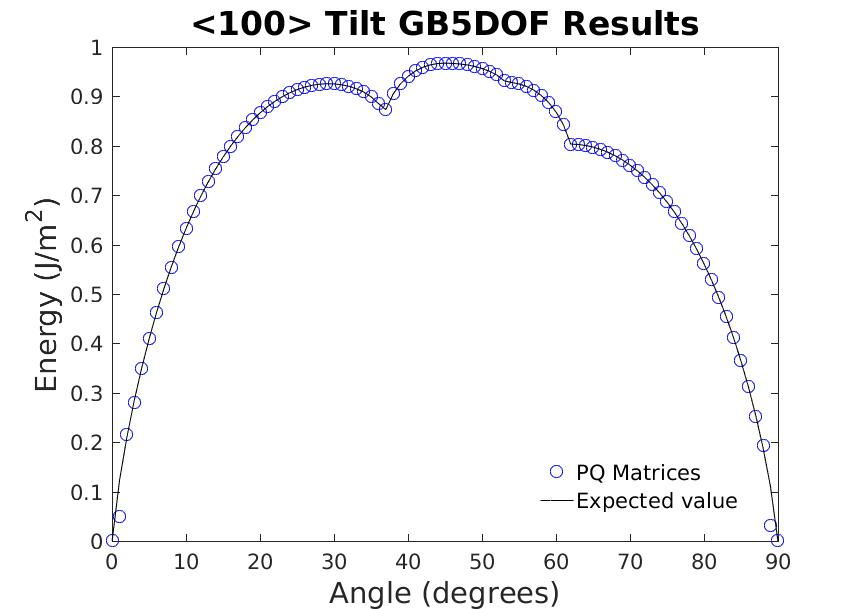
\includegraphics[scale=0.26]{Images/TestPQFit100Tilt}}
 \caption[A comparison of the \textlangle{}100\textrangle{} copper curves with the calculated results.]{\label{appfig:compare100} The \textlangle{}100\textrangle{} twist \protect\subref{appfig:compare100Twist} and tilt \protect\subref{appfig:compare100Tilt} results for the P and Q matrices as compared to Bulatov \emph{et al.}'s energy profiles. Bulatov \emph{et al.}'s \lstinline!GB5DOF.m! MATLAB\textsuperscript{\textregistered} script calculated the expected values by using the default parameters.  The \lstinline!GB5DOF.m! script calculated the values using the generated matrices.  With the exception of the data points at 1\textdegree{} in both \protect\subref{appfig:compare100Twist} and \protect\subref{appfig:compare100Tilt} and 89\textdegree{} in \protect\subref{appfig:compare100Tilt}, the energies calculated from the matrices matches the expected curves exactly.}
\end{figure}

\begin{figure}[ht!]
 \centering
 
 \subfloat[]{\label{appfig:compare110Twist}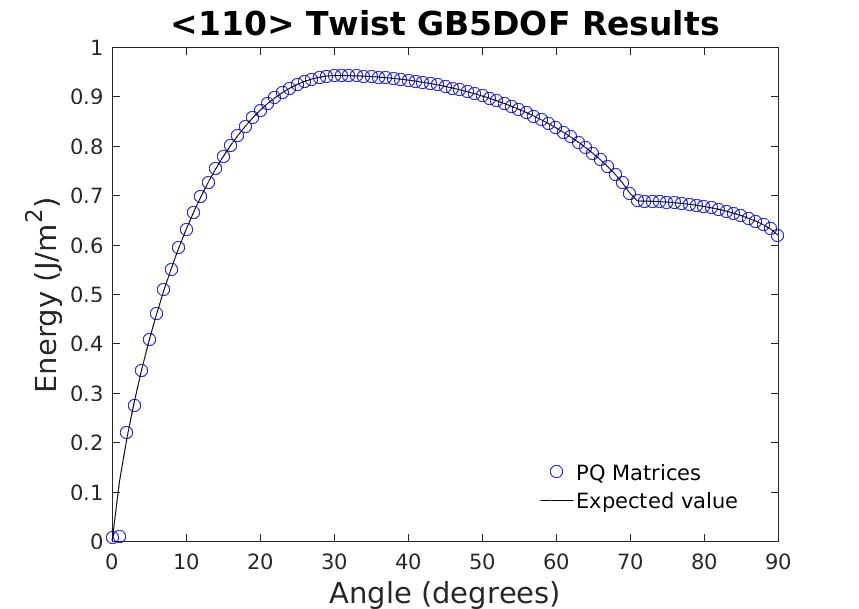
\includegraphics[scale=0.24]{Images/TestPQFit110Twist}}\quad
 \subfloat[]{\label{appfig:compare110Tilt}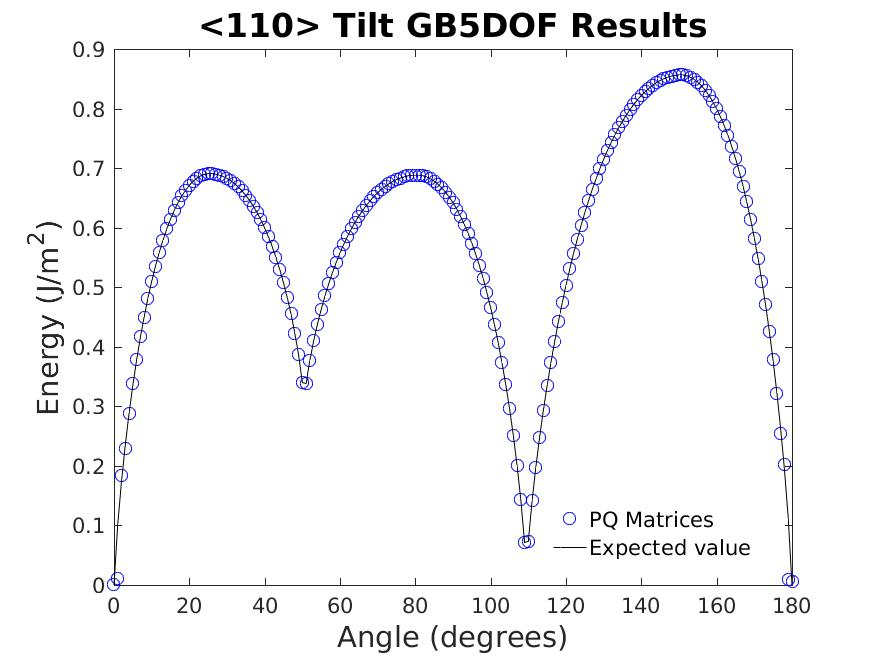
\includegraphics[scale=0.26]{Images/TestPQFit110Tilt}}
 \caption[A comparison of the \textlangle{}110\textrangle{} copper curves with the calculated results.]{\label{appfig:compare110} The \textlangle{}110\textrangle{} twist \protect\subref{appfig:compare110Twist} and tilt \protect\subref{appfig:compare110Tilt} results for the P and Q matrices as compared to Bulatov \emph{et al.}'s energy profiles. Bulatov \emph{et al.}'s \lstinline!GB5DOF.m! MATLAB\textsuperscript{\textregistered} script calculated the expected values by using the default parameters.  The \lstinline!GB5DOF.m! script calculated the values using the generated matrices. With the exception of the data points at 1\textdegree{} in both \protect\subref{appfig:compare110Twist} and \protect\subref{appfig:compare110Tilt} and 179\textdegree{} in \protect\subref{appfig:compare110Tilt}, the energies calculated from the matrices matches the expected curves exactly.}
\end{figure}

\begin{figure}[ht!]
 \centering
 
 \subfloat[]{\label{appfig:compare111Twist}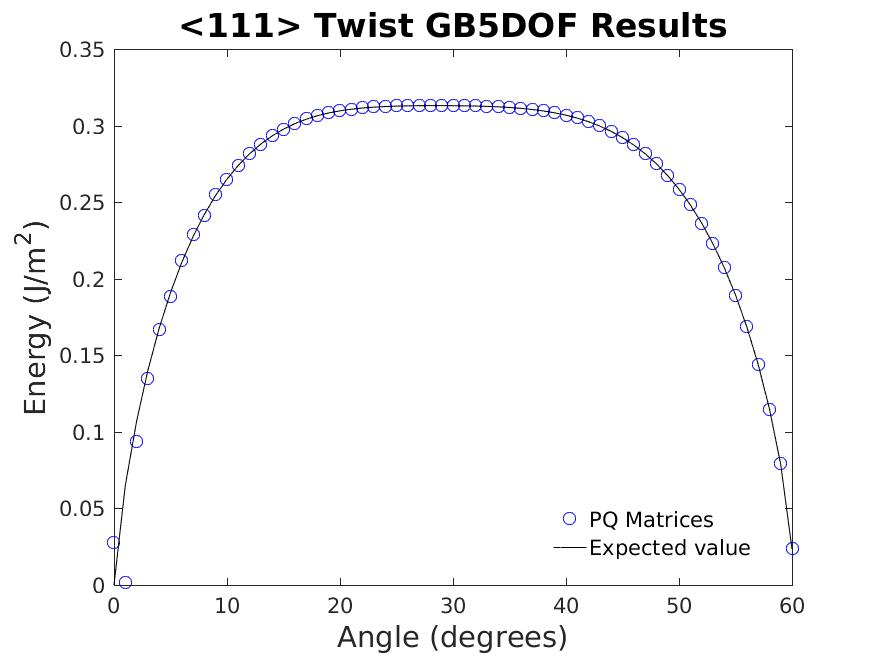
\includegraphics[scale=0.24]{Images/TestPQFit111Twist}}\quad
 \subfloat[]{\label{appfig:compare111Tilt}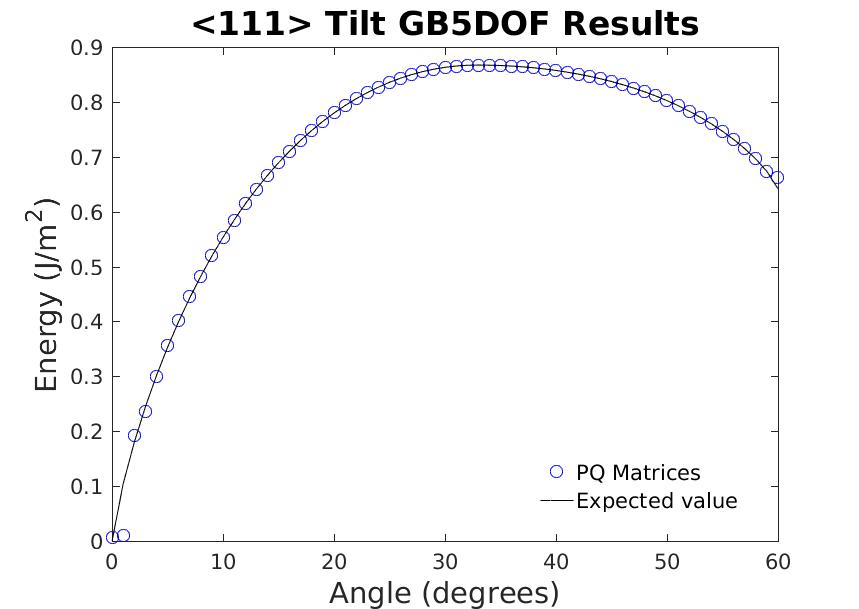
\includegraphics[scale=0.26]{Images/TestPQFit111Tilt}}
 \caption[A comparison of the \textlangle{}111\textrangle{} copper curves with the calculated results.]{\label{appfig:compare111} The \textlangle{}111\textrangle{} twist \protect\subref{appfig:compare111Twist} and tilt \protect\subref{appfig:compare111Tilt} results for the P and Q matrices as compared to Bulatov \emph{et al.}'s energy profiles. Bulatov \emph{et al.}'s \lstinline!GB5DOF.m! MATLAB\textsuperscript{\textregistered} script calculated the expected values by using the default parameters. The \lstinline!GB5DOF.m! script calculated the values using the generated matrices. With the exception of the data points at 1\textdegree{} in both \protect\subref{appfig:compare111Twist} and \protect\subref{appfig:compare111Tilt} and 60\textdegree{} in \protect\subref{appfig:compare111Tilt}, the energies calculated from the matrices matches the expected curves exactly.}
\end{figure}

\begin{figure}[ht!]
 \centering
 
 \subfloat[]{\label{appfig:100TwistPQ}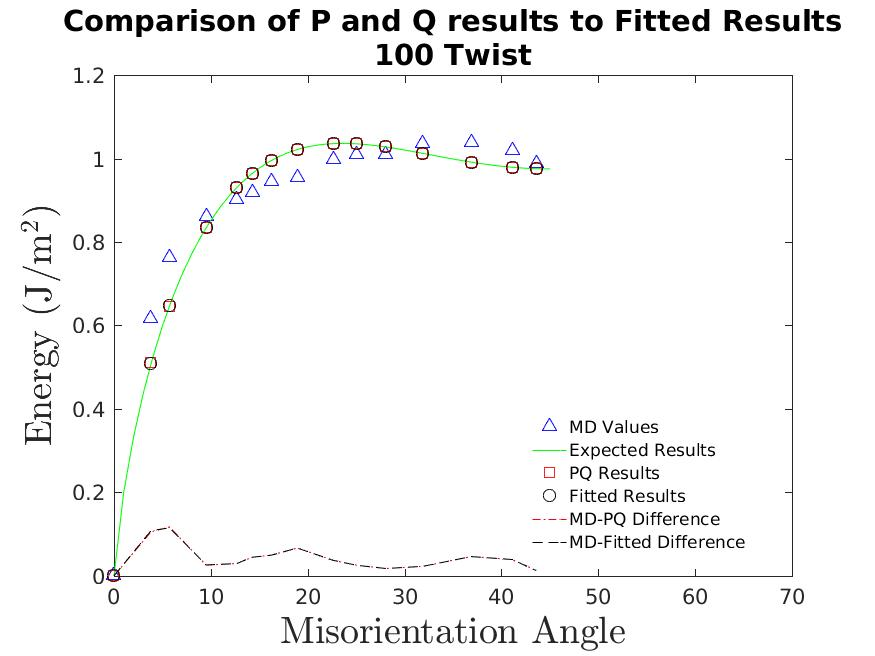
\includegraphics[scale=0.26]{Images/100TwistPQvsMD}}\quad
 \subfloat[]{\label{appfig:100TiltPQ}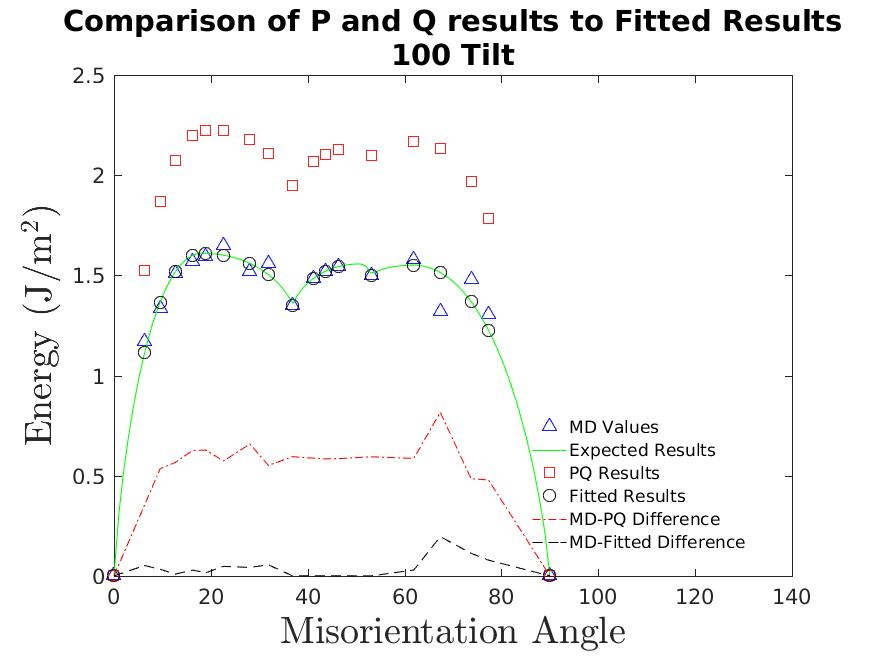
\includegraphics[scale=0.26]{Images/100TiltPQvsMD}}
 \caption[Comparison of the PQ matrices with the expected result for \textlangle{}100\textrangle{} 1D subset.]{\label{appfig:100PQ} A comparison of the expected value of the fitted function with the values calculated using the P and Q matrices for the \textlangle{}100\textrangle{} 1D subsets, with the MD values shown for reference.  \protect\subref{appfig:100TwistPQ} PQ results follow exactly the fitted curve.  \protect\subref{appfig:100TiltPQ} has a scaling issue yet to be fixed.  The cause of the scaling issue remains unknown.}
\end{figure}

\begin{figure}[ht!]
 \centering
 
 \subfloat[]{\label{appfig:110TwistPQ}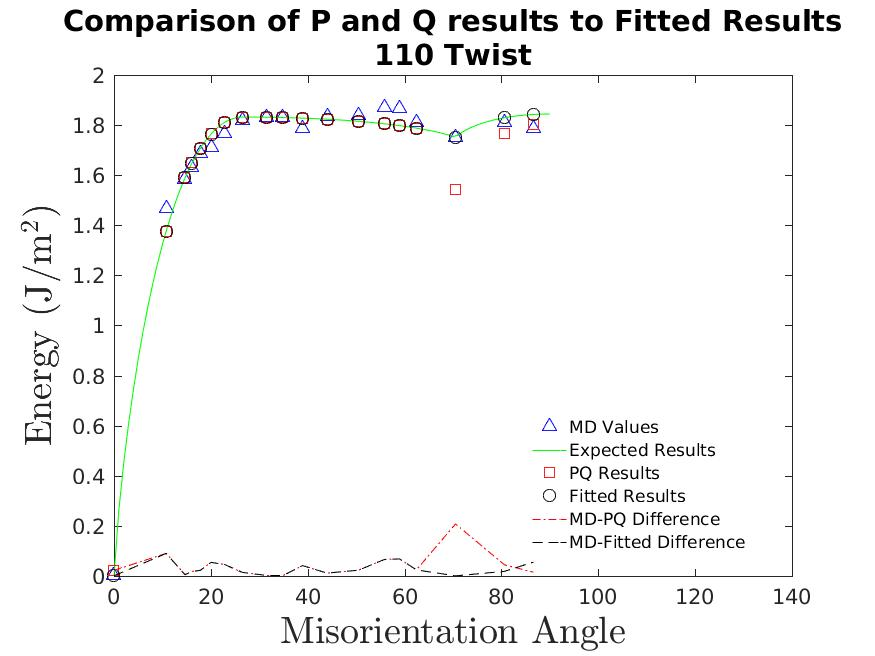
\includegraphics[scale=0.26]{Images/110TwistPQvsMD}}\quad
 \subfloat[]{\label{appfig:110TiltPQ}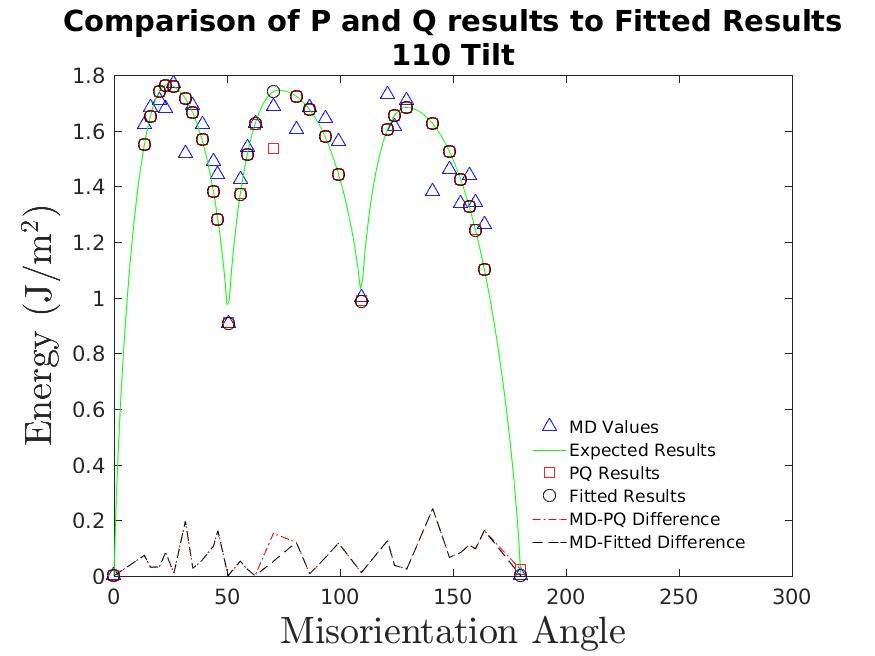
\includegraphics[scale=0.26]{Images/110TiltPQvsMD}}
 \caption[Comparison of the PQ matrices with the expected result for \textlangle{}110\textrangle{} 1D subset.]{\label{appfig:110PQ} A comparison of the expected value of the fitted function with the values calculated using the P and Q matrices for the \textlangle{}110\textrangle{} 1D subsets, with the MD values shown for reference.  \protect\subref{appfig:110TwistPQ} follows the fitted result until the cusp, at which point some anomalies appear.  The results from the PQ matrices dip well below the expected value at the cusp, and never make it back to the original fitted line. \protect\subref{appfig:110TiltPQ} has a similar issue on a lesser scale.  Only two of the calculated points do not follow the fitted curve.  At the endpoint the expected value is zero, but the PQ matrices calculated a value slightly higher.  Also, an unexpected cusp from the PQ matrices appears in the middle of the second hump.  All other data points follow the fitted curve exactly.}
\end{figure}

\begin{figure}[ht!]
 \centering
 
 \subfloat[]{\label{appfig:111TwistPQ}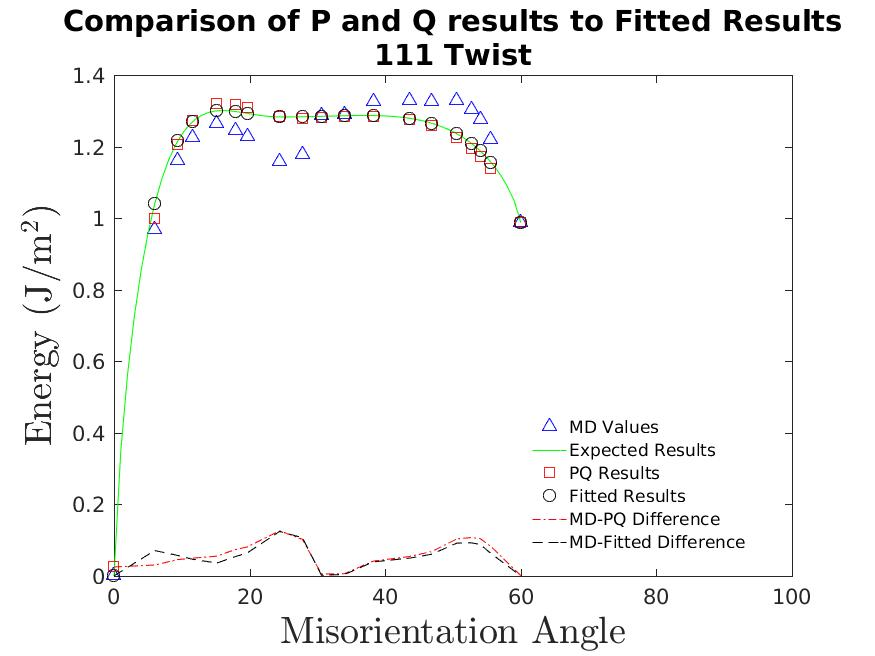
\includegraphics[scale=0.26]{Images/111TwistPQvsMD}}\quad
 \subfloat[]{\label{appfig:111TiltPQ}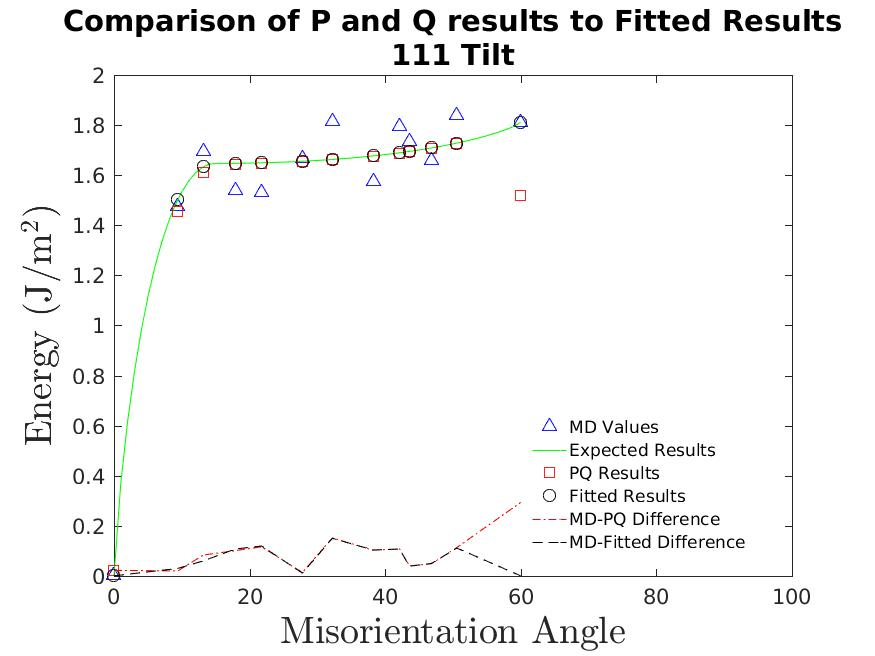
\includegraphics[scale=0.26]{Images/111TiltPQvsMD}}
 \caption[Comparison of the PQ matrices with the expected result for \textlangle{}111\textrangle{} 1D subset.]{\label{appfig:111PQ} A comparison of the expected value of the fitted function with the values calculated using the P and Q matrices for the \textlangle{}111\textrangle{} 1D subsets, with the MD values shown for reference.  \protect\subref{appfig:111TwistPQ} closely follows the expected fitted values, but has a slight error throughout.  \protect\subref{appfig:111TiltPQ} follows the expected values exactly in the center of the fitting, but misses slightly for lower angle boundaries, and misses completely at the end.}
\end{figure}

\chapter{Orientation Matrix Generator\label{app:OrientationMatrix}}
This code generates the orientation matrices (known as the P and Q matrices in Bulatov \emph{et al.}'s code). Provision for calculating the matrices one of two ways appears in-code through the use of command-line options.

\lstinputlisting[language=Python, breaklines=true, firstline=61]{../../scripts/orientation_matrix.py}

\chapter{Rotation Matrix Generator\label{app:RotationMatrix}}
This code generates the rotation matrices used to rotate the axes to the [100] direction as required by Bulatov \emph{et al.}'s script.

\lstinputlisting[language=Python, breaklines=true, firstline=25]{../../scripts/rotation_matrix.py}

\chapter{genOrientationMatrix.sh Bash Script\label{app:genOrientationMatrix}}
This bash script reads a CSV file containing misorientation angles data, and uses those angles to generate the P and Q matrices.  This script calls the script \lstinline!orientation_matrix.py!.

\lstinputlisting[language=Bash,breaklines=true]{../../scripts/genOrientationMatrices.sh}
\end{document}